\chapter{动态环境下的SLAM系统}
\label{sec:motion_segmentation}
动态分割(又称为移动物体检测/分割\cite{Derome2015Moving, Klappstein2008Moving, kundu2009movingA})透过将特征区分为两类特征,静态和动态特征,以检测图像中移动的区块。
明确地说,给定在图像空间中的特征点集合,动态分割将特征点聚类为静态集合和动态集合。
传统的视觉SLAM使用鲁棒的静态方法,计算几何模型(如基本矩阵、单应矩阵)来实现动态分割。
比如利用随机抽样一致算法(RANSAC)\cite{fischler1981randomA}和特定的距离度量方法(如桑普森距离\cite{Hartley2008Multiple})将不服从模型的点剔除。
当静态的特征点占了主体时,这种方法能够有很好的效果。
当动态物体占了相机的绝大部份, 或是捕捉到的场景被巨大的移动物体遮挡时,这种方法可能就会失败。
其他方法结合其他传感器来解决这个问题,如使用惯性测量单元(IMU)估计相机自身的运动\cite{Jones2011Visual, Leutenegger2014Keyframe}。
通过IMU得到的位姿估计可以用来初始化相机位姿并且鲁棒地分割静态和动态特征。
在这一章节,我们讨论传统视觉SLAM和视觉惯性SLAM之外,分割静态和动态物体的其他方法。

\section{背景--前景初始化}
背景-前景初始化技术假设系统有对于环境的先验知识,利用这个信息分割静态和动态特征。这个先验知识可以归于背景( 静态特征)或是前景( 动态特征)。
如果系统的先验知识是关于前景目标,表示系统知道相机前方运动物体的类型或形状。

\begin{figure}[thbp]
	\centering
	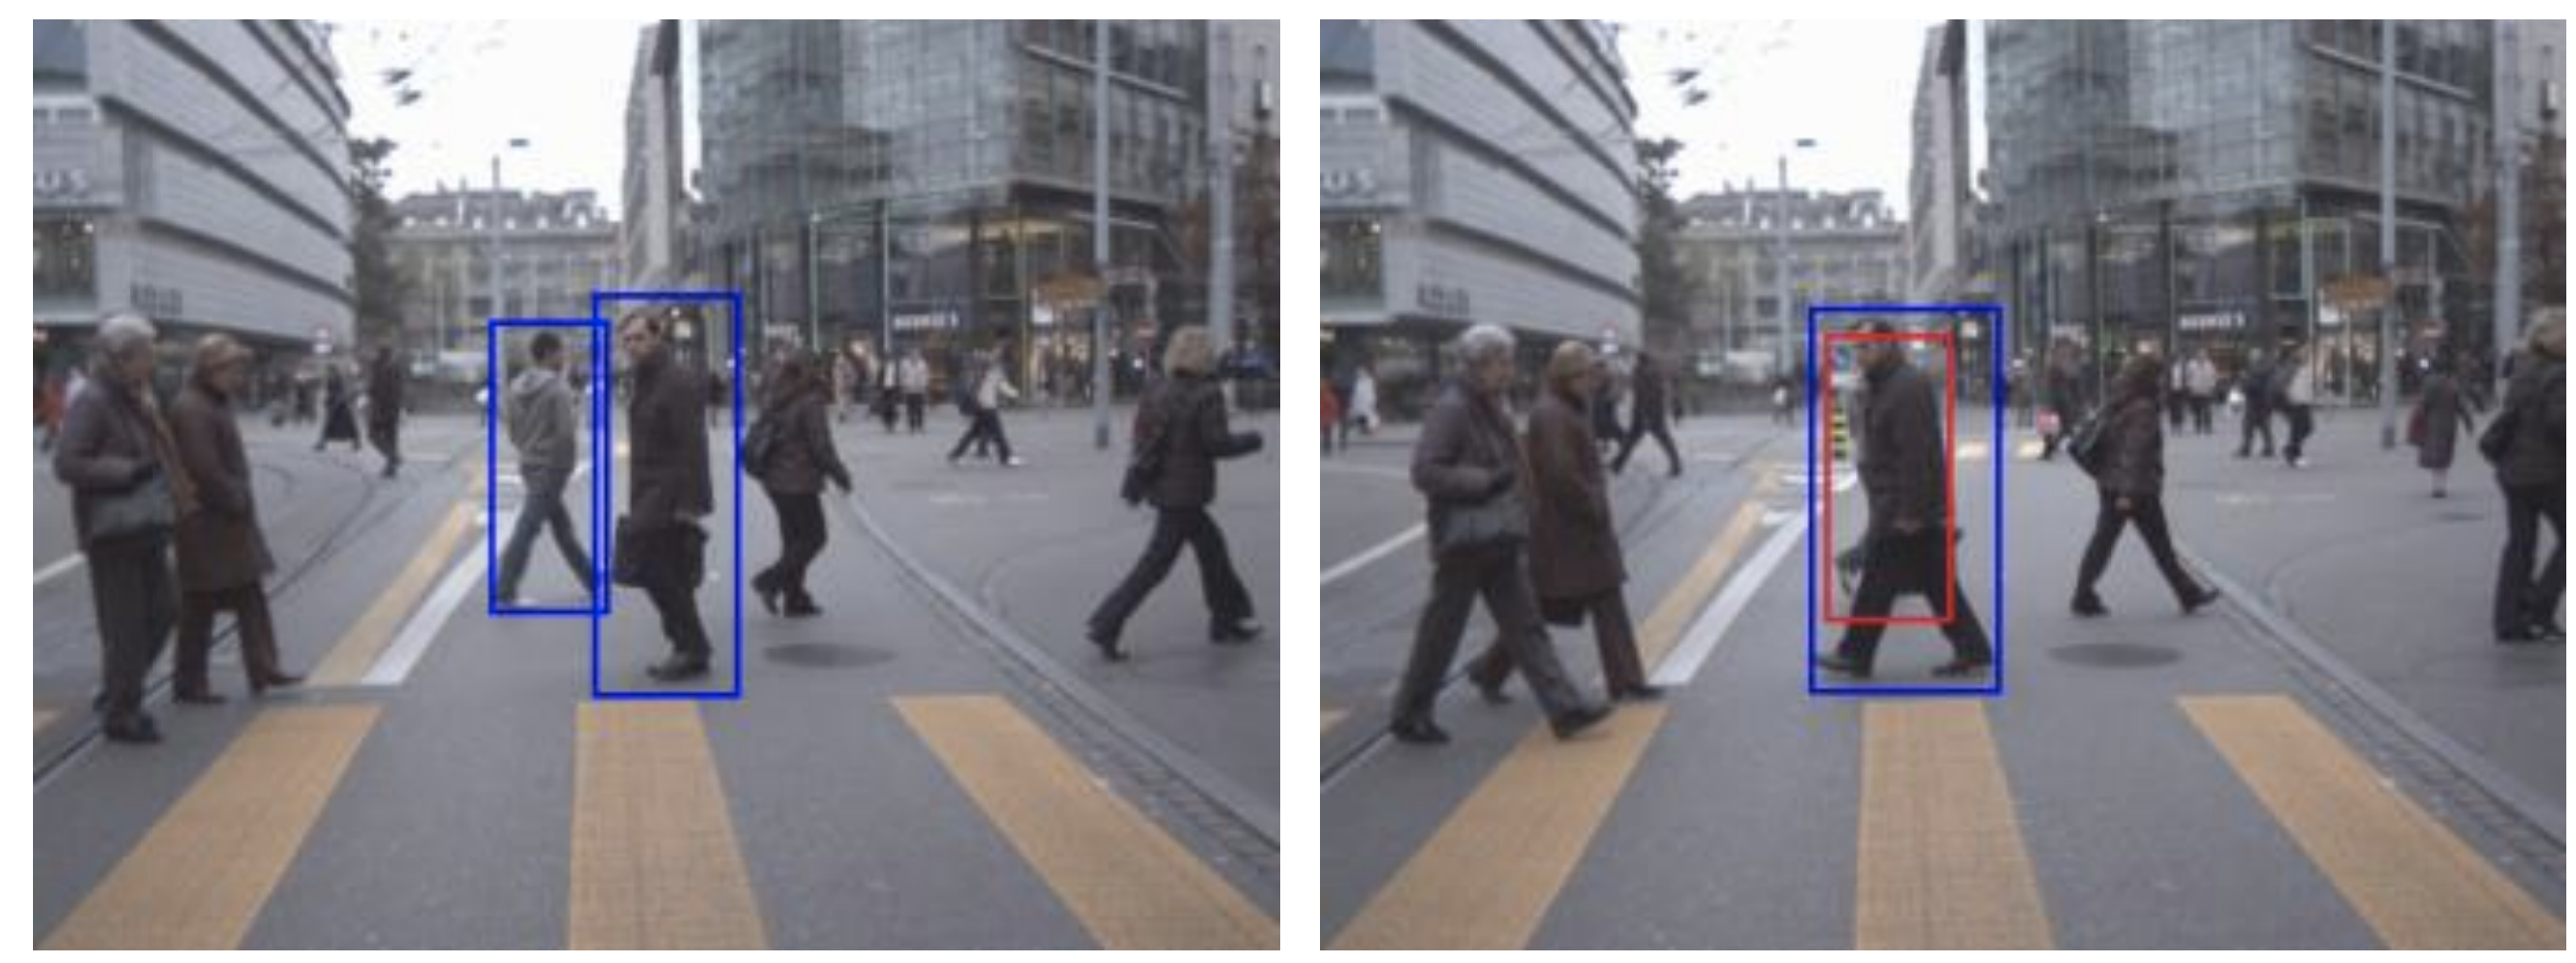
\includegraphics[width=0.9\textwidth]{figs/1-1/tbd.png}
	\caption{Tracking-by-detection~\cite{Breitenstein2010Online}示意图。蓝色框内为检测结果,红色框内为预测的匹配结果。}
	\label{fig:tracking_by_detection}
\end{figure}

大部分前景初始化的实现方法使用tracking-by-detection结构\cite{Breitenstein2010Online, Lee2014Driving},如图\ref{fig:tracking_by_detection}所示。Wangsiripitak等人\cite{Wangsiripitak2009Avoiding}假设对于一个三维物体,它的动态特征的位置是已知的。他们用边上的控制点集建模一个三维多面体模型,然后使用Harris’s RaPid tracker\cite{Harris1990RAPID}对其进行跟踪。如果之前跟踪的特征位于跟踪中的三维多面体上,当检测到这个物体处于移动状态时,便将特征剔除。被这个物体遮挡的静态特征也会被剔除。相似地,Wang等人\cite{Wang2010Visual}假设移动中的物体上的SURF特征描述子\cite{Bay2008Speeded}是已知的并存在数据库中。通过比较在特征检测步骤得到的描述子,就可以识别移动中的物体,也可以估算它的位移和旋转。Chhaya等人\cite{Chhaya2016Monocular}使用deformable wireframe object class model对建模相机前方的车辆。这个模型使用Principal Component Analysis (PCA) 在3D CAD data上训练而得。这个模型用在位姿估计得过程将车子识别并分割出来。另一方面,Lee等人\cite{Lee2014Driving, Lee2016Ground}基于tracking-by-detection结构,他们使用Constrained Multiple-Kernel(CMK)法,利用深度信息处理跟踪过程中的遮挡问题,同时使用预训练的人类检测器来跟踪行人。

有别于初始化前景的物体,背景初始化采用背景提取(background subtraction)技术 \cite{Babaee2017A,Piccardi2005Background}, 如图\ref{fig:bgsub}所示。Zhang等人\cite{Zhang2012Visual}初始化属于背景的特征点集合,并令这个集合为背景的模型。他们假设当首次进行视觉的初始化时,是没有前景物体的。当经过新的一帧后,使用GPCA\cite{Ren2005Generalized}进行三维动态分割。分割出来的动态部分,对于先前的背景模型具有最高响应值部分,将会用来更新背景。根据新的背景模型,运用标准的对极几何法估计位姿。

\begin{figure}[thbp]
	\centering
	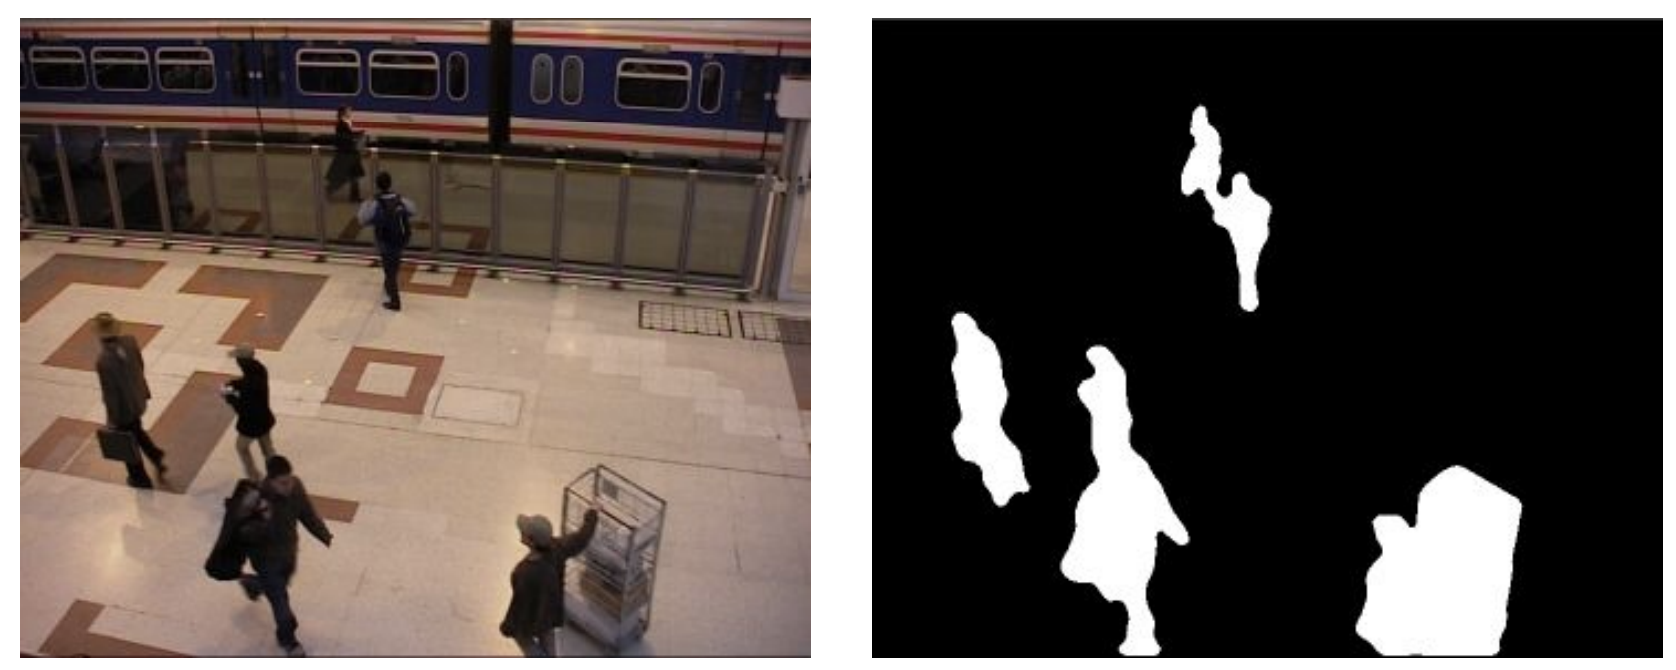
\includegraphics[width=0.9\textwidth]{figs/1-1/subback.png}
	\caption{基于~\cite{Babaee2017A}的背景提取结果。}
	\label{fig:bgsub}
\end{figure}

\section{基于几何约束的运动分割}
由于动态的特征会违反静态场景中的多视角几何约束,依赖此约束的技术是利用极限几何的性质\cite{Hartley2008Multiple}来分割静态和动态特征。这些约束可以从极线、三角化、基本矩阵估计或重投影误差的等式中得出。


Kundu等人\cite{kundu2009movingA}根据机器人里程计构建一个基本矩阵来定义两个几何约束。第一个约束是极线几何约束,在随后的视角下,成功匹配的点应该要在对应的极线上。如果跟踪到的特征离极线过远,就会被认为是动态特征。第二个约束是Flow Vector Bound(FVB),目的是分割当三维点沿着极线移动时产生的退化运动。通过设定跟踪到的特征流的上界和下界,超过这个范围的特征就会被作为运动的特征检测出来。最后通过循环的贝叶斯滤波器决定将特征分类为静态特征或动态特征。不同于使用极线约束,Migliore等人\cite{Migliore2009Use}利用三角化的原理分割静态和动态特征。他们在概率滤波器的框架下,持续地检查三个不同视角投影出来的视线的交点。如果特征是动态的,则这个交点在运动的过程中不会一样,甚至不会产生交点。但是由于传感器存在的噪声,他们使用Uncertain Projective Geometry\cite{Heuel2001Matching},将测量的不确定性加入他们检查不同视线关系的过程。最后通过统计方式分类静态和动态的特征。

将移动的物体误分类为静态物体并将其加入位姿估计,将会严重地使SLAM系统的性能降低,Lin等人\cite{Wang2007Simultaneous}通过观察这一性质来检测移动中的物体。他们计算两种不同条件下的位姿估计之间的差异,其中一个不加入新检测到的特征,另外一个假设新检测到的特征是静态的并加入位姿估计。借由计算两个结果的距离,设定一个门槛,通过二分贝叶斯滤波器整合,就能够精确地分割静态和动态的特征。

另外一个几何的方法是利用重投影误差。Zou和Tan\cite{Danping2013CoSLAM}将先前帧的特征投影到当前帧上,测量这些跟踪到到特征的距离。通过这个重投影的距离分类静态和动态的特征。Tan等人\cite{Wei2013Robust}使用同样的投影原理检测动态特征。他们同时将遮挡问题作为考量提出了一个鲁棒的视觉SLAM。在一个特征投影到当前帧上时,他们检测图像上的外观差异,也就是图像中的某一部分是否改变了。如果外观差异巨大,有极大的可能这个区域被动态物体遮挡,或是因为视点改变被静态物体所遮挡。因为上述原因被遮挡的三维点,会被保留并用来估算相机位姿。

\section{基于光流的运动分割}
光流的定义了两个连续的图像间,图案亮度的表面运动\cite{Horn1980Determining}。通常它对应了图像的运动场,因此可以用于分割移动的物体。Klappstein\cite{Klappstein2008Moving}根据光流定义了运动度量描述移动中的物体的似然。测量当场景中有运动物体时,光流错误的范围。Graph-cut算法根据运动度量分割移动的物体。

Alcantarilla等人\cite{Alcantarilla2012On}通过运动似然残差得到的场景流(三维的光流)中的三维运动向量系数,分割移动物体。马氏距离用于考量基于稠密光流和双目重建计算场景流的测量不确定性。如果残差小,特征点很可能属于静态物体。在运动似然残差设立门槛,属于运动物体的特征点可以从SLAM过程中删除,使得视觉里程计的估计更鲁棒。Derome等人\cite{Derome2015Moving, Derome2014Real}计算预测的预想与双目相机观测得到的图像的残差,以此计算光流。预测的图像是根据估计的相机自身运动,将当前帧的双目图像转换到过去的帧上。接着从残差场上的斑点检测移动中的物体。

\section{相机运动约束}
一般的SfM和视觉SLAM通过8点的均值\cite{Longuet1981A}或5点法\cite{David2004An}计算相机的运动。这种普通的相机运动估计并没有考虑任何相机移动方式的假设。另外一种方式是假设相机根据特定参数提供的外在信息(如车轮里程计的信息)估计相机位姿。加入这种相机运动约束,通过匹配特征点是否符合相机运动的约束,分类静态特征。

Scaramuzza\cite{scaramuzza20111A}提出利用轮式车辆的非完整性约束计算相机运动的方法。他假设相机运动是平面或圆形的,以此建模相机运动。由此约束,相机运动可以被参数化为1自由度并且可由1点法计算\cite{scaramuzza2009realA}。同样地,Sabzevari等人\cite{sabzevari2016multiA}也利用阿克曼转向几何提供的轮式车辆约束来计算相机运动。满足估计的相机运动的特征点会被认为是静态特征,其他的特征点则被认为是动态特征。
